%医学物理实验_实验报告

%文档类型
\documentclass[a4paper,12pt]{article}%A4纸,默认字体大小为12pt(小四),文档类型为论文

%宏包
%文字设置
\usepackage[UTF8,heading = true]{ctex}%处理中文
\usepackage{xeCJK}%处理中文
\usepackage{fontspec,xunicode,xltxtra}%字体设置
%文档&排版设置
\usepackage{titlesec}%自定义章节标题样式
\usepackage{multicol}%分栏
\usepackage{hyperref}%超链接设置\daleth 
\usepackage{multirow,makecell}%制作复杂表格
\usepackage{booktabs}%画三线表要用
\usepackage{float}%图片、表格等位置浮动排版
\usepackage{indentfirst}%首行缩进
\usepackage{graphicx,subfigure}%图片插入
\usepackage{listings}%代码高亮
\usepackage{xcolor}
\usepackage{appendix}%附录
\usepackage{fancyhdr}%页眉页脚
\usepackage{geometry}%页边距
\usepackage{caption}
\usepackage{setspace}%局部行距设置
%数学
\usepackage{amsmath,amssymb}%公式
\usepackage{amsfonts,mathrsfs}%数学字体
\usepackage{fontspec}%字体包
\setmainfont{Times New Roman}%让全文英文字体为新罗马字体,同样地,也可以用这种方法改字体为Arial等
%数学字体中起冲突的包为 txfonts, txfonts包的作用是使得全文为 times new roman 字体
%!!!这样英文字体就被锁死,再也无法变动!!!
%解决方法也很简单,调用包时,amsmath一定要在 txfonts包前面
\usepackage{array}%矩阵
\usepackage{gensymb}%角度单位“度”的命令:~\degree 

\geometry{a4paper,scale=0.8}%设置了纸张为a4,并且版心占页面长度的比例为80%;scale也可以改为ratio,表示版面边距占页面长度的比例. 
\hypersetup{colorlinks=true,linkcolor=black,citecolor=black}%去掉目录等超链接所带的红框,并让参考文献的引用颜色为黑色
\setlength{\parindent}{2em}%首行缩进2字符
\lstset{
    columns=fixed,
    numbers=left, % 在左侧显示行号
    numberstyle=\footnotesize\color{darkgray},% 设定行号格式
    backgroundcolor=\color[RGB]{245,245,244},% 设定背景颜色
    keywordstyle=\color[RGB]{40,40,255},% 设定关键字颜色
    numberstyle=\color[RGB]{0,192,192},%行号数字样式
    commentstyle=\it\color[RGB]{0,96,96},% 设置代码注释的格式
    stringstyle=\rmfamily\slshape\color[RGB]{128,0,0},% 设置字符串格式
}
\pagestyle{fancy}%页眉页脚
\fancyhead{}%清空页眉
\fancyhead[R]{\zihao{-5}{\leftmark}}%页眉右侧为section名(subsection命令为“\rightmark”)
\fancyhead[L]{\zihao{-5}{医学物理实验:实验报告}}%页眉左侧为标题

%章节名称样式
\CTEXsetup[format={\centering\zihao{3}\heiti}]{section}%设置章标题字号为Large,居中
\CTEXsetup[name={第,章}]{section}%第*章
\CTEXsetup[number={\chinese{section}}]{section}%计数器名称为“section”;chinese格式的序号一,二,三,..

\CTEXsetup[format={\centering\zihao{-3}\heiti}]{subsection}
\CTEXsetup[name={第,节}]{subsection}%第*节                            
\CTEXsetup[number={\chinese{subsection}}]{subsection}%计数器名称为“subsection”

\CTEXsetup[format={\zihao{4}\heiti}]{subsubsection}
\CTEXsetup[name={,、}]{subsubsection}%*、
\CTEXsetup[number={\chinese{subsubsection}}]{subsubsection}%计数器名称为“subsubsection”

%修改目录、参考文献标题样式
\renewcommand\contentsname{\hfill {\zihao{-2}{\heiti 目录}} \hfill}%目录标题居中,用\hfill填充两侧空白

%中英摘要
\newcommand{\enabstractname}{\Large Abstract}%标题
\newcommand{\cnabstractname}{\Large \heiti 摘要}%标题
\newenvironment{enabstract}{%
  \par\small
  \noindent\mbox{}\hfill{\bfseries \enabstractname}\hfill\mbox{}\par
  \vskip 2.5ex}{\par\vskip 2.5ex}
\newenvironment{cnabstract}{%
  \par\small
  \noindent\mbox{}\hfill{\bfseries \cnabstractname}\hfill\mbox{}\par
  \vskip 2.5ex}{\par\vskip 2.5ex}

\newcommand{\suo}{\indent}%缩进2个字符

\title{{\zihao{4}{大学物理-综合实验B\\医学物理实验\\实验报告}}\\\footnotesize{College Physics Comprehensive Experiment B\\Medical Physics Experiment: Experimental Report}}%标题
\author{
    \small 李佩哲\\
    \small 指导教师:顾悦\\
    \footnotesize 中国科学技术大学~生命科学与医学部~生命科学学院\\
    \footnotesize 230026\\
    \footnotesize 安徽~合肥}
\date{\small\today}

\setlength{\headheight}{15pt}%为了解决默认字号设为12pt而引发的某些警告

\begin{document}

\maketitle%标题(封面)
\thispagestyle{empty}%不显示页眉页脚

\newpage%分页
\thispagestyle{empty}%不显示页眉页脚
\begin{center}
    \section*{\hfill \heiti{大学物理-综合实验B} \hfill}%用\hfill填充两侧空白
    \section*{\hfill \heiti{实验基本信息} \hfill}%用\hfill填充两侧空白
\end{center}

\begin{table}[H]
    \begin{center}
        \begin{tabular}{|c|c|}%分四列,每列之间、两边都划竖线(用符号“|”表示);c意为居中
            \hline %划一条一整行的横线
                \textbf{\heiti{~实验人}}&李佩哲~~~PB21051049\\
            \hline
                \textbf{\heiti{~~~~~~实验名称~~~~~~}}&医学物理实验:温度传感器特性及人体温度测量实验\\
            \hline
                \multicolumn{2}{|c|}{\textbf{\heiti{研究背景及意义}}}\\
            \hline
                \multicolumn{2}{|c|}{\makecell{\\\parbox{16.8cm}
                {~~~~~~~在医学上,体温的测量及温度的误 差对疾病的判断相当重要,所以温度传感器应用广泛.~~因此,对温度传感器的工作原理、使用方法进行实验探究很有必要.~~}\\~}}\\
            \hline
                \multicolumn{2}{|c|}{\textbf{\heiti{研究内容}}}\\
            \hline
                \multicolumn{2}{|c|}{\makecell{\\\parbox{16.8cm}
                {\begin{enumerate}
                    \item 了解实验中使用的温度传感器的工作原理,测量所使用的温度传感器的电压(或电阻)与温度的关系,求出温度传感器的灵敏度与相关系数;
                    \item 用选用的温度传感器、放大电路和数字电压表组装数字式电子温度表,并用标准数 字式温度表,对组装的数字式温度表进行校正,通过实验测量其线性度;
                    \item 使用组装的数字式温度表进行人体各部位温度分布情况的测量, 了解人体各部分的温差.~~
                \end{enumerate}
                }\\~}}\\
                
            \hline
                \multicolumn{2}{|c|}{\textbf{\heiti{研究计划}}}\\
            \hline
                \multicolumn{2}{|c|}{\makecell{\\\parbox{16.8cm}
                {测量温度传感器的输出特性;\\
                制作数字式电子温度表并进行定标,计算其线性度.~~}\\~}}\\
            \hline
                \multicolumn{2}{|c|}{\textbf{\heiti{预期研究成果}}}\\
            \hline
                \multicolumn{2}{|c|}{\makecell{\\\parbox{16.8cm}
                {深入了解温度传感器工作原理,对其电路结构有一定的了解;\\
                学习掌握各类温度传感器与温度关系式及其推论,学会进行温度计线性度分析.~~}\\~}}\\
            \hline
        \end{tabular}
    \end{center}
\end{table}

\newpage%分页
\thispagestyle{empty}%不显示页码
\begin{spacing}{1.528}%段落行距设置
\begin{cnabstract}%中文摘要
    医学上,体温的测量及温度的误差对疾病的判断相当重要,因此温度传感器应用广泛.~~本实验通过测量温度传感器的输出特性、制作数字式温度表并进行定标,加深了对温度传感器工作原理与特性的理解与掌握.~~
    \\\textbf{关键词:}温度、传感器、LM35温度传感器
\end{cnabstract}

\begin{enabstract}%英文摘要
    In medicine, the measurement of body temperature and the error of temperature are very important for the judgment of diseases, so temperature sensors are widely used. By measuring the output characteristics of the temperature sensor, making a digital thermometer and calibrating, this experiment has deepened the understanding and grasp of the working principle and characteristics of the temperature sensor.
    \\\textbf{Keywords:}temperature, sensor, LM35 temperature sensor
\end{enabstract}
\end{spacing}

\newpage%分页
\thispagestyle{empty}%不显示页眉页脚
\tableofcontents%生成目录
\thispagestyle{empty}%不显示页眉页脚
\newpage
\setcounter{page}{1}%从这开始标页码
%\begin{multicols}{2}%分栏

\section{绪论}%一级标题
\subsection{实验背景}
\begin{spacing}{1.528}%段落行距设置
“温度”是一种重要的热学物理量,它不仅和我们的生活环境密切相关,在科研及生产过程中,温度的变化对实验及生产的结果至关重要,所以温度传感器应用广泛.~~
温度传感器可以提高温度控制精度,提高了控制效率,从而有效地提高仪器仪表测量分析性能
$^\text{\cite{应用1}}$;
也可以基于温度传感器实现的电动机过载保护
$^\text{\cite{应用2}}$;
等等.~~
在医学上,体温的测量及温度的误差对疾病的判断相当重要.~~
\end{spacing}

\subsection{实验目的和意义}
\begin{spacing}{1.528}%段落行距设置
    \begin{enumerate}
        \item 了解实验中使用的温度传感器的工作原理,测量所使用的温度传感器的电压(或电 阻)与温度的关系,求出温度传感器的灵敏度与相关系数;
        \item 用选用的温度传感器、放大电路和数字电压表组装数字式电子温度表,并用标准数 字式温度表,对组装的数字式温度表进行校正,通过实验测量其线性度;
        \item 使用组装的数字式温度表进行人体各部位(眉心,手心等)温度分布情况的测量, 了解人体各部分的温差.~~
    \end{enumerate}
\end{spacing}

\subsection{实验方法}
\begin{spacing}{1.528}%段落行距设置
借助医学物理实验箱,探究给定的LM35温度传感器的输出特性,并利用其构建电路,组装数字式电子温度表,通过与标准温度计进行比较来定标,然后测量并计算组装温度计的线性度即可.~~
\end{spacing}

\section{实验原理}
\subsection{热敏电阻温度传感器}
\subsubsection{恒压源电流法测量热电阻}
\begin{spacing}{1.528}%段落行距设置
串联已知电阻$R_1$与热电阻$R_t$,分别测量二者的电压$U_{R_1},U_{R_t}$,则热电阻阻值可以表示为$R_t=\frac{U_{R_t}}{U_{R_!}}R_1$
$^\text{\cite{讲义}}$.

\subsubsection{负温度系数热敏电阻(NTC 1K)温度传感器}
在一定的温度范围内(小于150~\degree  C)NTC 热敏电阻的电阻$R_t$与温度$T$之间的关系为$R_t=R_0e^{B\left(\frac{1}{T}-\frac{1}{T_0}\right)}$,
从而$\ln R_t=B\left(\frac{1}{T}-\frac{1}{T_0}\right)+\ln R_0$.
作$\ln R_t-\frac{1}{T}$直线图,用直线拟合,由斜率 即可求出常数 B
$^\text{\cite{讲义}}$.~~
\end{spacing}

\subsection{PN结温度传感器}
\begin{spacing}{1.528}%段落行距设置
通常 PN 结组成二极管的电流$I$和电压$U$满足$I=I_s\left[e^{\frac{qU}{kT}}-1\right]$,常温时$I=I_se^{\frac{qU}{kT}}$.~~在正向电流保持恒定且电流较小条件下,近似有$U=BT+$Ugo
$^\text{\cite{讲义}}$.
\end{spacing}

\subsection{LM35 集成电压型温度传感器}
\begin{spacing}{1.528}%段落行距设置
由于LM35温度传感器输出的是与温度对应的电压(10~mV/\degree  C),且线性极好,故只要配上电压源,数字式电压表就可以构成一个精密数字测温系统.~~
输出电压的温度系数$K=$10.0~mV/\degree  C,因此可以通过测量电压求得被测温度$T=\frac{U_0}{K}$
$^\text{\cite{讲义}}$.~~
\end{spacing}

\section{实验仪器}
\begin{spacing}{1.528}%段落行距设置
温度传感器特性及人体温度测量实验仪由 7 部分组成
$^\text{\cite{讲义,实验}}$:
\begin{enumerate}
\item 高准确度控温恒温加热系统;
\item 直流稳压电源;
\item 数字电压表;
\item Pt100 温度传感器;
\item NTC1K 热敏电阻温度传感器、 PN 结温度传感器、电压型集成温度传感器 LM35及可调放大器;
\item 标准数字体温表;
\item 实验接插线.~~
\end{enumerate}
\end{spacing}

\section{实验过程}
\subsection{测量温度传感器的输出特性$^\text{\cite{讲义}}$}
\begin{spacing}{1.528}%段落行距设置
    按面板电路图指示插好实验电路,将控温传感器 Pt100 铂电阻插入干井式恒温加热炉的中心井,另一只待测试的热敏电阻插入干井式恒温加热炉另一井,
    然后开启控温仪开关.~~ 从 30.0~\degree  C起,每隔 10.0~\degree  C设置控温系统温度,待控温稳定后,记录温度传感器的输出,
    到 80.0~\degree  C止.~~对测量结果进行处理,拟合求出温度传感器的灵敏度与相关系数.~~
\end{spacing}

\subsection{制作数字式电子温度表$^\text{\cite{讲义}}$}
\begin{spacing}{1.528}%段落行距设置
    \begin{enumerate}
        \item 将控温传感器 Pt100 铂电阻插入恒温加热炉中心井,控温仪作 37.0~\degree  C的自适应整定.
        \item 用数字体温计作为标准温度表,对控温仪 Pt100 铂电阻进行 37.0~\degree  C温度校正.~~\\
                控温仪设定 37.0~\degree  C,对比控温仪实际温度示数与数字体温表示数.~~如不同,进行传感器修正.
        \item 测量组装数字式电子温度计的线性度.~~\\
                从 35.0~\degree  C~42.0~\degree  C,每隔1~\degree  C设置控温仪温度,到 42.0~\degree  C止,
                分别记录组装数 字式电子温度计和标准温度表的温度示数,求出不同设定温度时的差值∆t,计算线性度.~~ 
        \item 使用组装的数字式电子温度计进行人体温度测量.~~\\
        用组装数字式电子温度计,进行人体各部位的温度测量,
                了解人体各部位温差的原因.~~
    \end{enumerate}
\end{spacing}

\section{实验数据与处理}
\subsection{实验数据}
实验数据整理如下.~~原始记录见附件.
\begin{table}[H]
    \begin{minipage}{0.25\linewidth}
        \centering
        \begin{tabular}{cc}
            \toprule
            $T$/\degree C & $U$/V \\
            \midrule
            30.2 	&	0.291 	\\
            40.1 	&	0.397 	\\
            50.1 	&	0.504 	\\
            60.0 	&	0.600 	\\
            70.1 	&	0.710 	\\
            80.0 	&	0.811 	\\
            \bottomrule
        \end{tabular}
        \caption{温度传感器特性}\label{1}
    \end{minipage}
    \begin{minipage}{0.49\linewidth}  
        \centering
        \begin{tabular}{cccc} 
            \toprule
            $\frac{\text{控温仪}}{\text{\degree C}}$ & $\frac{\text{组装温度计}}{\text{\degree C}}$ & $\frac{\text{标准温度计}}{\text{\degree C}}$ & $\Delta T$/\degree C\\
            \midrule
                35.0 	&	35.0 	&	34.8 	&	+0.2	\\
                36.0 	&	36.0 	&	36.0 	&	0.0	\\
                37.0 	&	37.0 	&	37.0 	&	0.0	\\
                38.0 	&	38.1 	&	38.1 	&	0.0	\\
                39.0 	&	39.2 	&	39.1 	&	+0.1	\\
                40.0 	&	40.2 	&	40.3 	&	-0.1	\\
                41.0 	&	41.3 	&	41.3 	&	0.0	\\
                42.0 	&	42.3 	&	42.3 	&	0.0	\\
            \bottomrule
        \end{tabular}
        \caption{制作数字式电子温度表}\label{2}
    \end{minipage}
    \begin{minipage}{0.25\linewidth}
        \centering
        \begin{tabular}{cc}
            \toprule
            手心/\degree C & 手背/\degree C \\
            \midrule
                36.1&34.4\\
            \bottomrule
        \end{tabular}
        \caption{测量人体各部位体温}\label{3}
    \end{minipage}
\end{table}

\subsection{实验数据处理}
\subsubsection{温度传感器的输出特性}
\begin{spacing}{1.528}%段落行距设置
    由表\ref{1}中数据绘制图象如图\ref{11}所示,求得拟合直线为$y = 0.0104x - 0.0217$,相关系数$r^2 = 0.9998$,
    因此温度传感器的灵敏度为0.0104,相关系数为0.9998.
\end{spacing}

\begin{figure}[H]
    \centering
    \subfigure[温度传感器的输出特性]{\label{11}
        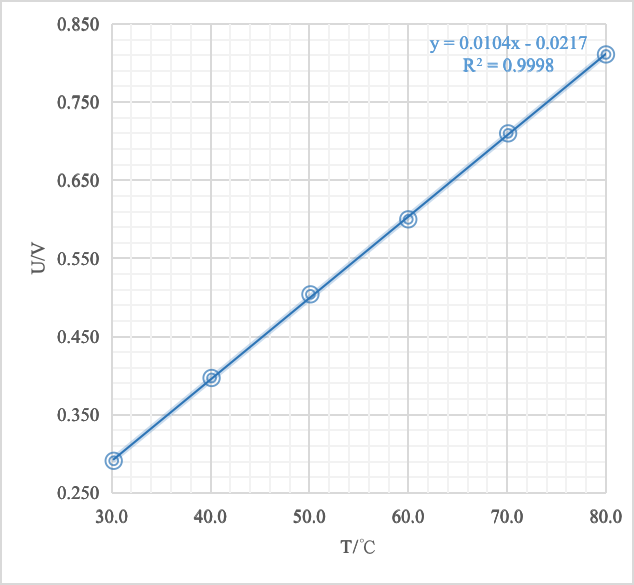
\includegraphics[scale=0.55]{特性.png}
        }
    \quad
    \subfigure[制作数字式电子温度表]{\label{22}
        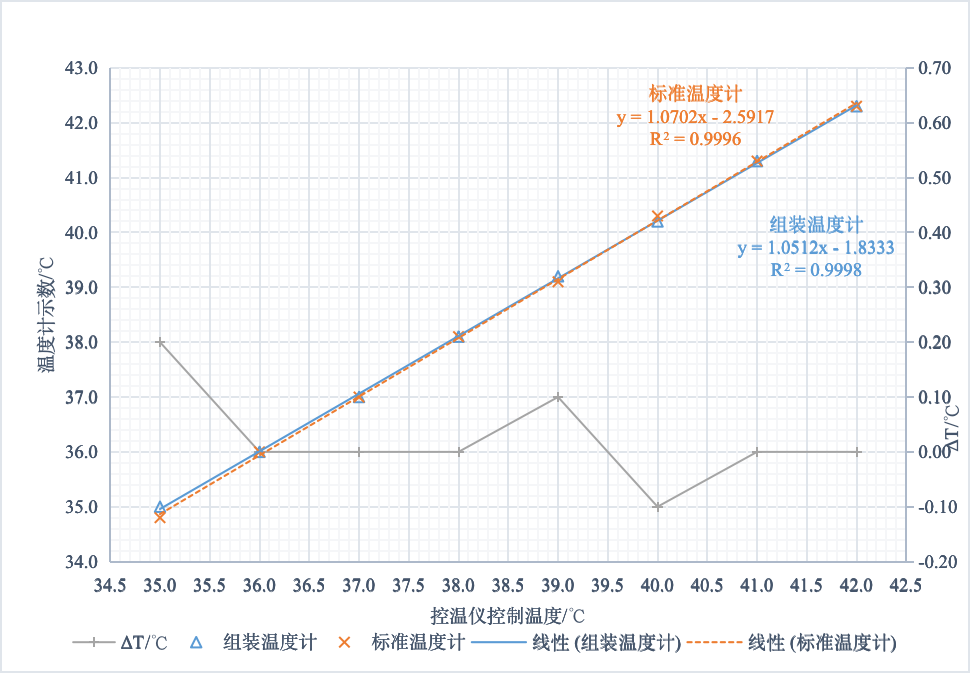
\includegraphics[scale=0.6]{制作.png}
        }
    \caption{实验结果}\label{水滴接触角图}
\end{figure}

\subsubsection{制作数字式电子温度表}
\begin{spacing}{1.528}%段落行距设置
    由表\ref{2}中数据绘制图象如图\ref{22}所示,求得最大偏差$Y_{\max} \approx \Delta T_{\max}=0.2$~\degree C,满量程输出$Y=T_{\max}-T_{\min}=42.3\text{~\degree C}-35.0$\degree C$=7.3$~\degree C,
    因此电子温度计的线性度$\delta=\frac{Y_{\max}}{Y}\times 100\%=\frac{0.2}{7.3}\times 100\%\approx2.74\%$.
\end{spacing}

\subsubsection{人体温度测量}
\begin{spacing}{1.528}%段落行距设置
    由表\ref{3}中数据可知,人手掌心温度显著高于手背温度.
\end{spacing}

\section{结论}
\begin{spacing}{1.528}%段落行距设置
    根据以上结果与数据处理,可以得到如下结论:
    \begin{enumerate}
        \item LM35温度传感器的输出一般为线性,其灵敏度为0.0104,相关系数为0.9998;
        \item 制作的数字式电子温度计具有良好的测温性能,与标准温度计相差无几,且其线性度可达约2.74\%;
        \item 人体手掌心温度显著高于手背温度,可能的原因有:与手掌开放式的结构相比,手心较为封闭的结构使得热量更难散失;手掌心处的毛细血管比手背处的更为发达,带来了更多的热量;等.
    \end{enumerate}
\end{spacing}

\section{结语}
\begin{spacing}{1.528}%段落行距设置
    本实验系统探究了LM35温度传感器的输出特性,对相关理论进行了学习与探讨,并利用其特性制作了数字式电子温度计,进行定标并实际应用;
    但还存在一些不足之处,比如研究的对象为LM35温度传感器,而对热敏电阻温度传感器如NTC~1K温度传感器、PN结温度传感器没能进行深入而系统的研究;
    再比如实验步骤还能进一步优化,但碍于实验者的能力水平,未能取得较为深刻的进展,等等. 
    希望后续的研究者能够借鉴本课题的成果与不足,拓展研究面,细化理论模型,改进实验步骤,进而取得更加深入的突破. 
\end{spacing}

\section{致谢}
\begin{spacing}{1.528}%段落行距设置
    本实验为笔者大雾实验的收官之作,在此笔者郑重感谢本门课程对笔者自身实验水平的提高做出的卓越贡献。
    与此同时,笔者还要向本门课程的实验老师们(尤其是本实验的指导老师——顾悦老师)致以崇高的敬意与深深的感谢。
    正是实验老师们的兢兢业业、耐心细致的指导,让笔者能够顺利完成各项实验,取得个人能力的提升。
    笔者在此向在课程过程中向笔者提供帮助的老师们和同学们致以由衷的感谢!
\end{spacing}

\newpage
\begin{thebibliography}{23}%不使用BibTeX的方法;99意为参考文献的最大数值为99个,这个数可以自己设置
    \bibitem{应用1}李香宇,任建存,王世功,徐向美.基于LM35的高精度温控系统的设计[J].电子设计工程,2017,25(15):94-97.DOI:10.14022/j.cnki.dzsjgc.2017.15.024.
    \bibitem{应用2}徐进.基于LM35D的电动机过载保护的设计和实现[J].机床电器,2000(03):44-45.
    \bibitem{讲义}中国科大物理实验预约选课系统. 医学物理实验[EB/OL]. (2022-09-01)[2022-10-18]. http://pems.ustc.edu.cn/uploads/project/20221003/0a7d4af229a8081e98bb9454e26cb67c.pdf
    \bibitem{实验}朱小松.集成温度传感器LM35制作的数字温度计[J].电子技术应用,1991(10):25.
\end{thebibliography}

\begin{appendices}
\section*{附录~~~实验数据记录}
\begin{spacing}{1.528}%段落行距设置
    见附件.~~
\end{spacing}
\end{appendices}

\end{document}